\documentclass[12pt]{article}
%\usepackage{amsmath}
\usepackage{graphicx}
%\usepackage{enumerate}
\usepackage{natbib} %comment out if you do not have the package
\usepackage{url} % not crucial - just used below for the URL 
\usepackage{amsmath, amssymb}
\usepackage{setspace} % NOT IN TECHNOMETRICS TEMPLATE
\usepackage{caption} % NOT IN TECHNOMETRICS TEMPLATE



%\pdfminorversion=4
% NOTE: To produce blinded version, replace "0" with "1" below.
\newcommand{\blind}{0}

% DON'T change margins - should be 1 inch all around.
\addtolength{\oddsidemargin}{-.5in}%
\addtolength{\evensidemargin}{-.5in}%
\addtolength{\textwidth}{1in}%
\addtolength{\textheight}{1.3in}%
\addtolength{\topmargin}{-.8in}%

\date{}
\begin{document}

%\bibliographystyle{natbib}

\def\spacingset#1{\renewcommand{\baselinestretch}%
{#1}\small\normalsize} \spacingset{1}


%%%%%%%%%%%%%%%%%%%%%%%%%%%%%%%%%%%%%%%%%%%%%%%%%%%%%%%%%%%%%%%%%%%%%%%%%%%%%%

\if0\blind
{
  \title{\bf Combining model calibration and design}
  \author{Carl Ehrett\thanks{
    The authors gratefully acknowledge \textit{please remember to list all relevant funding sources in the unblinded version}}\hspace{.2cm}\\
    School of Mathematical and Statistical Sciences, Clemson University,\\
    D. Andrew Brown \\
    School of Mathematical and Statistical Sciences, Clemson University,\\
    Evan Chodora \\
    Department of Mechanical Engineering, Clemson University,\\
    Christopher Kitchens \\
    Department of Chemical and Biomolecular Engineering, Clemson University,\\
    and \\
    Sez Atamturktur \\
    Department of Architectural Engineering, Pennsylvania State University\\}
  \maketitle
} \fi

\if1\blind
{
  \bigskip
  \bigskip
  \bigskip
  \begin{center}
    {\LARGE\bf Title}
\end{center}
  \medskip
} \fi

\bigskip
%\begin{abstract}
%Abstract
%\end{abstract}

\noindent%
{\it Keywords:}  
\vfill

\newpage
\spacingset{2} % DON'T change the spacing!
\section{Introduction}
\label{introduction}

%
The goal of traditional Kennedy-O'Hagan style calibration \citep[KOH, ][]{kennedy2001} is to find a posterior distribution on unknown parameters by calibrating a computer model using real-world observations of the modeled phenomenon.
%
By contrast, the design methodology of calibration to target outcomes (CTO) uses the KOH framework to find a posterior distribution on optimal input settings in the model by ``calibrating'' a computer model using artificial observations that reflect performance and cost targets for the modeled system.
%
The goal of the work described here is to combine KOH and CTO.
%
Call the resulting methodology DCTO, for dual calibration to target outcomes.

CTO as previously developed assumes, somewhat idealistically, that the computer model is already perfectly calibrated.
%
DCTO avoids this idealization.
%
Furthermore, when undertaking KOH, some areas of the model range may be of greater interest than others.
%
For example, one may be more interested in calibrating the model to be accurate in the optimal region of some design variable $\theta$ than elsewhere.
%
Undertaking dual calibration may allow us to focus our calibration efforts on such regions of interest, prioritizing them over other areas of the model range.
%

\section{The model}

%
Let $f$ be the model of interest, and partition its inputs as $(x,\theta_1,\theta_2)$ where $x$ denotes the known and/or controllable inputs, $\theta_1$ denotes the parameters targeted for KOH calibration, and $\theta_2$ denotes the input settings targeted for design via CTO.
%
If $f$ can be run quickly, then we use it directly in MCMC.
%
However, if it is computationally expensive, we employ a surrogate by setting a Gaussian process (GP) prior on $f$ with mean $m_0(x,t_1,t_2)$ and covariance function $C_0((x,t_1,t_2),(x',t_1',t_2'))$.
%
From here on in this discussion, assume that a GP surrogate is used for $f$.
%
Typically, there will be some systematic discrepancy between the output of $f$ and the true system, even if the true value of $\theta_1$ is used.
%
We model this discrepancy, between the true system and $f$ at the true value of $\theta_1$, with another GP prior $\delta_1$ having mean $m_1(x,t_2)$ and covariance function $C_1((x,t_2),(x',t_2'))$.
%
In addition to the discrepancy between $f$ and the true system, there may also be a systematic discrepancy between the true system and our performance/cost targets, particularly if the latter are especially optimistic.
%
We model this discrepancy using a GP prior with mean $m_2(x)$ and covariance function $C_2(x,x')$.
%
Notice that this discrepancy is between the true system at optimal settings for $\theta_2$ and $f$ using the true value of $\theta_1$ and the optimal settings for $\theta_2$.
%
In addition to systematic discrepancy between $f$ and reality, measurement error must be included in the model.
%
Thus let $\epsilon\sim N(0,\sigma^2)$ denote the (known) i.i.d.\ variance of (real) observations at any given values of $x,t_2$.
%
Finally, we assume that $\eta,\delta_1,\delta_2,$ and $\epsilon$ are all mutually independent.
%

%
A collection of simulation runs is needed to train the GP code surrogate.
%
Let $(\mathbf{x_s},\mathbf{t_{1s}},\mathbf{t_{2s}})$ be the design matrix for these simulation runs, and let $\mathbf{y_s}$ denote the output of these runs.
%
Similarly, let $\mathbf{y_r}$ be the real observations at $\mathbf{x_r},\mathbf{t_{2r}}$, and let $\mathbf {y_d}$ be a set of artificial ``observations'' reflecting our cost and performance targets at control settings $\mathbf {x_d}$.
%
Call $\mathbf{y_d}$ the {\em target outcomes}.
%
Finally, let $\mathbf y = (\mathbf{y_s},\mathbf{y_r},\mathbf{y_d})^T$.
%
Then it follows that $\mathbf y\sim \mathrm{N}(\mathbf m,\mathbf C)$, where
\[
\mathbf m = \begin{pmatrix}
m_0(\mathbf{x_s},\mathbf{t_{1s}},\mathbf{t_{2s}})\\
m_0(\mathbf{x_r},\mathbf1\theta_1,\mathbf{t_{2r}}) + m_1(\mathbf{x_1},\mathbf{t_{2r}})\\
m_0(\mathbf{x_d},\mathbf1\theta_1,\mathbf1\theta_2) + m_1(\mathbf{x_d},\mathbf1\theta_2) + m_2(\mathbf{x_d})
\end{pmatrix},
\]
\[
\mathbf C = \begin{pmatrix}
\mathbf{C_{11}} & \mathbf{C_{12}} & \mathbf{C_{13}}\\
\mathbf{C_{21}} & \mathbf{C_{22}} & \mathbf{C_{23}}\\
\mathbf{C_{31}} & \mathbf{C_{32}} & \mathbf{C_{33}}
\end{pmatrix},
\]
\begin{align*}
\mathbf{C_{11}}&=C_0\left((\mathbf{x_s},\mathbf{t_{1s}},\mathbf{t_{2s}}),(\mathbf{x_s},\mathbf{t_{1s}},\mathbf{t_{2s}})\right)\\
\mathbf{C_{21}}&=C_0\left((\mathbf{x_s},\mathbf{t_{1s}},\mathbf{t_{2s}}),(\mathbf{x_r},\mathbf1\theta_1,\mathbf{t_{2r}})\right)\\
\mathbf{C_{31}}&=C_0\left((\mathbf{x_s},\mathbf{t_{1s}},\mathbf{t_{2s}}),(\mathbf{x_d},\mathbf1\theta_1,\mathbf1\theta_2)\right)\\
\mathbf{C_{12}}&=\mathbf{C_{21}}^T\\
\mathbf{C_{22}}&=C_0\left((\mathbf{x_r},\mathbf1\theta_1,\mathbf{t_{2r}}),(\mathbf{x_r},\mathbf1\theta_1,\mathbf{t_{2r}})\right) + C_1\left( (\mathbf{x_r},\mathbf{t_{2r}}),(\mathbf{x_r},\mathbf{t_{2r}}) \right) + \sigma_2 \mathbf I\\
\mathbf{C_{32}}&=C_0\left((\mathbf{x_r},\mathbf1\theta_1,\mathbf{t_{2r}}),(\mathbf{x_d},\mathbf1\theta_1,\mathbf1\theta_2)\right) + C_1\left( (\mathbf{x_r},\mathbf{t_{2r}}),(\mathbf{x_d},\mathbf1\theta_2) \right)\\
\mathbf{C_{13}}&=\mathbf{C_{31}}^T\\
\mathbf{C_{23}}&=\mathbf{C_{32}}^T\\
\mathbf{C_{33}}&=C_0\left((\mathbf{x_s},\mathbf1\theta_1,\mathbf1\theta_2),(\mathbf{x_s},\mathbf1\theta_1,\mathbf1\theta_2)\right) + C_1\left( (\mathbf{x_s},\mathbf1\theta_2),(\mathbf{x_s},\mathbf1\theta_2) \right) + C_2(\mathbf{x_d},\mathbf{x_d})
\end{align*}
%
Note that when $\mathbf{y_d}$ and $\mathbf{x_d}$ are empty and $\mathbf m, \mathbf C$ reduce respectively to their first two and upper two-by-two block elements, this is simply the KOH framework.
%
Thus, DCTO generalizes the KOH framework.
%

%
\section{Example with simulated data}
%
Consider the function of three inputs $f(x,t_1,t_2) = x / (t_2^{t_1-1}\exp(-0.75t_2)+1)$. 
%
Figure \ref{fig:example_output} shows the output of this function for $x=1$ over the range $(t_1,t_2)\in[1.5,4.5]\times[0,5]$.
%
\begin{figure}
\centering
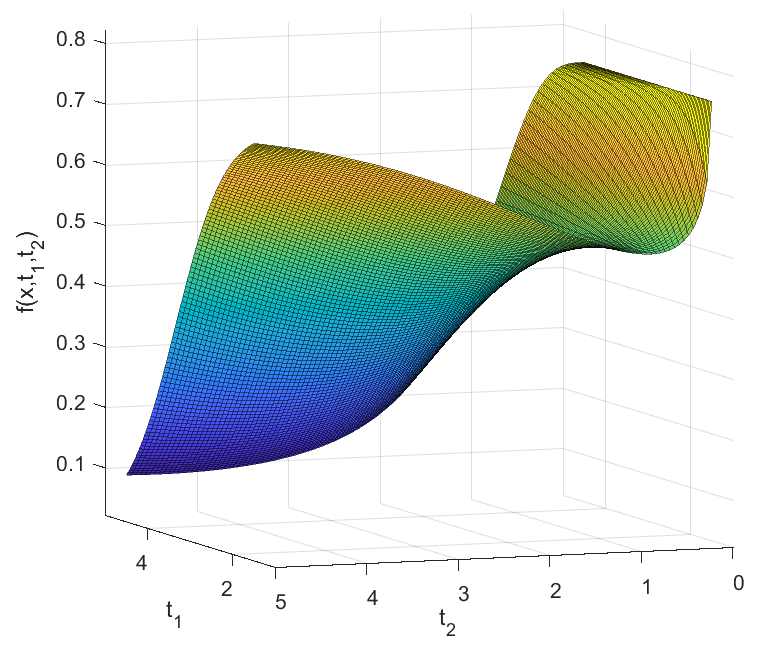
\includegraphics[scale=0.85]{FIG_obj_fn}
\captionsetup{width=.85\linewidth}
\caption{Example computer model output over the support of the calibration parameter $t_1$ and the design parameter $t_2$.}
\label{fig:example_output}
\end{figure}
%
We arbitrarily set $\theta_1=2$ to be the ``true'' value of $t_1$.
%
For any value of $x$ and $t_1$, the optimal (minimizing) value of $t_2$ is $(4/3)(t_1-1)$, so we have $\theta_2=4/3.$
%
Figure \ref{fig:true_vals} shows the locations of the true and optimal values (respectively) of $\theta_1$ and $\theta_2$.
%
\begin{figure}
\centering
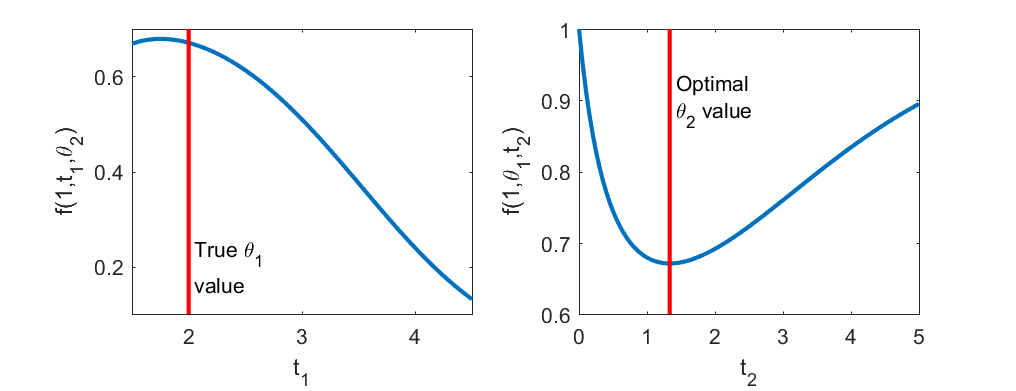
\includegraphics[scale=0.85]{FIG_true_optimal_theta1_theta2}
 	\captionsetup{width=.85\linewidth}
\caption{The lefthand plot shows the computer model output at $x=1$ and optimal $\theta_2$ for each value of the calibration parameter $t_1$ The righthand plot show the model output at $x=1,t_1=\theta_1$ for each value of the design parameter $t_2$.}
\label{fig:true_vals}
\end{figure}
%
There it is clear that the true value of $\theta_1$ is far from optimal -- if this value were within our control, its optimal value would be at the upper end of its support, at 4.5.
%
Thus $f$ showcases the ability of DCTO to perform simultaneously both calibration and design in the case when our ``truth-seeking'' goals and our design goals are in tension.
%

%
\subsection{Results}
% 
We used DCTO on four versions of the problem.
%
First, we assumed that $f$ is free from discrepancy -- i.e. that $f(x,\theta_1,t_2)$ is an unbiased estimator of the ``true'' system $g(x,t_2)$.
%
The other three versions each assume that $f$ suffers from some form of discrepancy.
%
Let $g_1,g_2,g_3$ denote the ``true'' systems in these three cases.
%
We set 
\begin{align*}
g_1(x,t_2) &= f(x,\theta_1,t_2) \left(1-c(x-.5)(x-1)/x) \right) \\
g_2(x,t_2)&= f(x,\theta_1,t_2) - c(x-.5)(x-1)\left(t_2-\frac43\right)^2 + d\\
g_3(x,t_2)&=f(x,\theta_1,t_2) + cxt_2+d
\end{align*}
%
Where $c,d$ are constants which determine how severe the discrepancy is in each case.
%
The function $g_1$ has a multiplicative discrepancy dependent only on $x$. 
%
This discrepancy does not affect the optimal value of $t_2$.  The discrepancy of $g_2$ is additive, and is dependent upon both $x$ and $\theta_1$. 
%
Though this discrepancy can affect the optimal value of $t_2$, in the case that $\theta_1=2$ (which is what we assume to be the truth) it does not.
%
Thus under $g_1$ and $g_2$, it remains the case that the optimal value of $t_2$ is $\theta_2=4/3$. 
%
By contrast, $g_3$ has an additive discrepancy which does affect the optimal setting for $t_2$. 
%
For $g_3$, optimal $t_2$ is dependent upon both the true value of $\theta_1$ and upon the value of $c$. 
%
For example, for $\theta_1=2$ and $c=0.055$, the optimal $t_2$ is $\theta_2\approx1$.
%
Figure \ref{fig:discrepancies} shows the discrepancies for two different versions (corresponding to different settings of $(c,d)$) of each $g_i$.
%
\begin{figure}
\centering
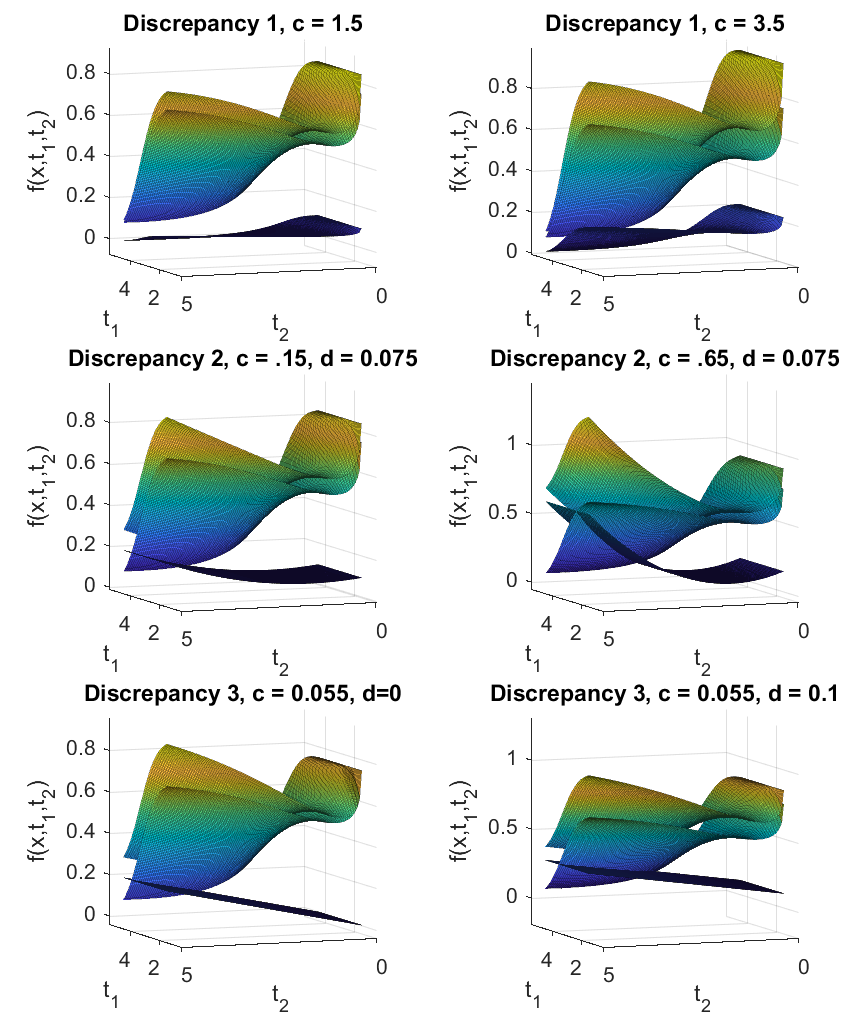
\includegraphics[scale=0.85]{FIG_six_discrepancies}
\captionsetup{width=.85\linewidth}
\caption{The $i^{\text{th}}$ row shows $g_i$ (the objective function with discrepancy), $f$ (the computer model), and the discrepancy $g_i-f$, all at $x=0.75$. In each row, a less aggressive version of the discrepancy appears on the left, and a more aggressive on the right. In each plot, the topmost surface is $g_i$, the middle surface is $f$, and the bottom surface is the discrepancy $g_i-f$.}
\label{fig:discrepancies}
\end{figure}
%

%
We applied DCTO to each of seven cases: the non-discrepancy case, and the two different versions of each $g_i$ shown in Figure \ref{fig:discrepancies}.
%
We found that in these cases, no appreciable difference resulted from the decision of whether or not to use an emulator (where the emulator was trained on a latin hypercube design of 250 points on the space of model inputs).
%
Therefore, the results reported here do not employ an emulator.
%
In each case, we gathered 50 ``observations'' of $g_i$ on a latin hypercube design over the supports of $x$ and $\theta_2$, setting $\theta_1$ equal to its ``true'' value of 2.
%
After standardizing the response to have mean 0 and standard deviation 1, we added i.i.d.\ N(0,0.05) noise to the response.
%
We then carried out DCTO using Metropolis-Hastings-within-Gibbs MCMC, drawing 8000 samples each of $t_1,t_2,\boldsymbol\rho_{\delta_1},\lambda_{\delta_1},\rho_{\delta_2},\lambda_{\delta_2}$, where the latter four are the hyperparameters of the product power exponential covariance functions $C_1$ and $C_2$.
%
In order to evaluate the success of the calibration component of DCTO, we also carried out a two-step procedure of using traditional KOH calibration of $\theta_1$, followed by a second step using CTO to obtain a distribution of $\theta_2$. 
%In the first step of this KOH+CTO procedure, we re-running the procedure with $\mathbf{x_d},\mathbf{y_d}$ as empty (null) vectors, followed by CTO calibration of $\theta_2$ using the 
%
The first step is essentially DCTO with $\mathbf{x_d},\mathbf{y_d}$ as empty (null) vectors, and the second step uses the distribution obtained in the first step to estimate $\theta_2$.
%
Thus, the comparison between DCTO and KOH+CTO shows the difference between DCTO and performing CTO on a system which has been calibrated using traditional methods.
%
%In doing so, we would hope to find that DCTO and KOH give similar posterior distributions for $\theta_1$, and that DCTO gives a posterior distribution of $\theta_2$ peaked at its optimal value while KOH gives a posterior distribution that approximates the (uniform) prior.
%
Figure \ref{fig:no_discrep_results} shows the results for $g_0$, the case of no discrepancy.
%
\begin{figure}
\centering
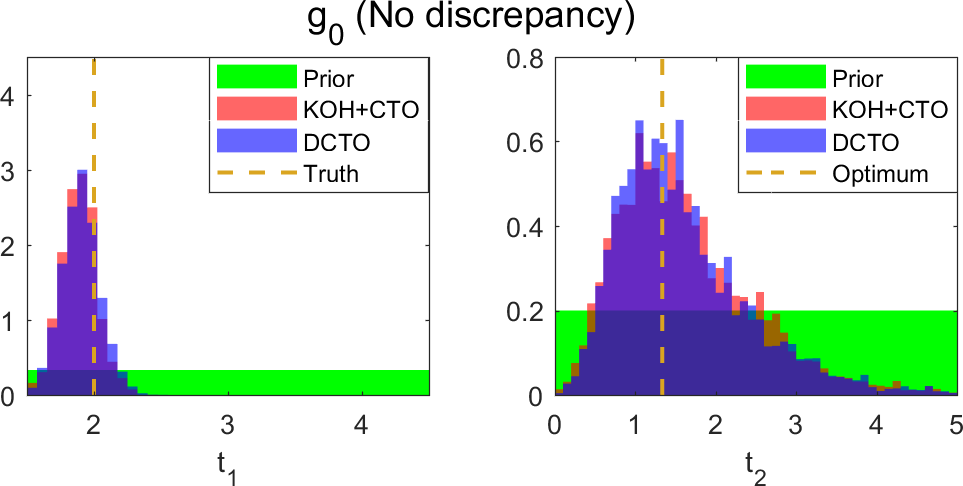
\includegraphics[scale=0.85]{FIG_KOHCTO_DCTO_comp_discrep0_results}
\captionsetup{width=.85\linewidth}
\caption{Prior and posterior distributions of the calibration parameter $\theta_1$ and design parameter $\theta_2$, along with their true/optimal values, for DCTO and KOH+CTO carried out when there is no discrepancy between the true system and the computer model.}
\label{fig:no_discrep_results}
\end{figure}
%
The two methods deliver comparable results, showing that combining KOH calibration and CTO design into DCTO does not undermine the performance of either task.
%
Strong Bayesian learning has occurred for both parameters, in that the posterior distributions of $\theta_1,\theta_2$ are peaked around their true and optimal values, respectively.
%
KOH gives a similar posterior for $\theta_1$, showing that the expansion of DCTO to undertake design has not interfered with its calibration performance.
%
The skewness apparent in the posterior distributions of $\theta_2$ occur in all of the results gathered here, and is likely due to the shape of the objective function $f$, which increases sharply for $t_2<\theta_2$ and increases much more gently for $t_2>\theta_2$.
%

%
Figure \ref{fig:1_discrep_results} shows the results for $g_1$ at two settings of $c$, and Figure \ref{fig:2_discrep_results} shows the results for $g_2$ at two settings of $(c,d)$.
%
\begin{figure}
\centering
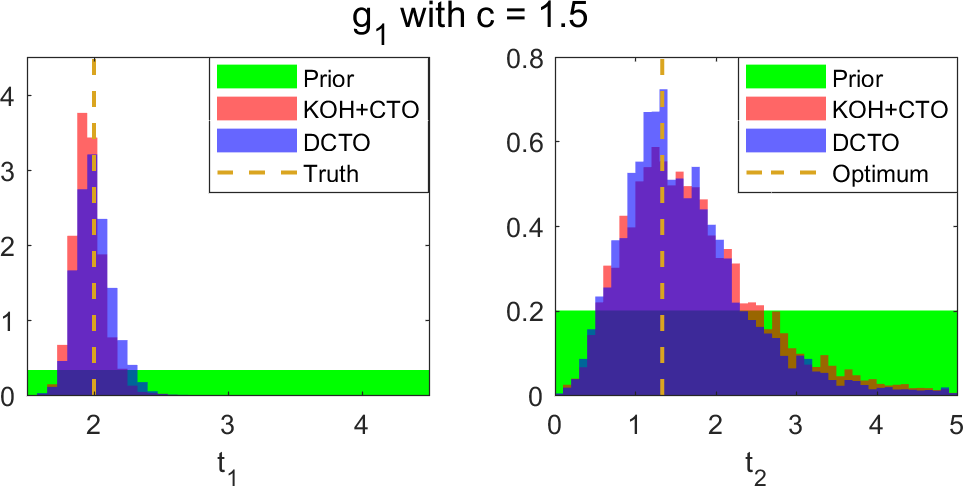
\includegraphics[scale=0.85]{FIG_KOHCTO_DCTO_comp_discrep1_results}
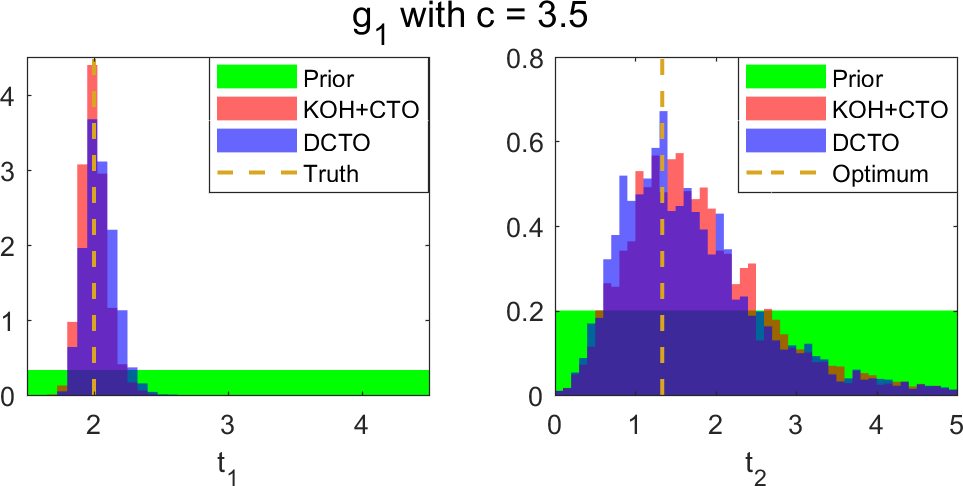
\includegraphics[scale=0.85]{FIG_KOHCTO_DCTO_comp_discrep2_results}
\captionsetup{width=.85\linewidth}
\caption{Prior and posterior distributions of the calibration parameter $\theta_1$ and design parameter $\theta_2$, along with their true/optimal values, for DCTO and KOH+CTO in the case of true systems $g_1$. The top row corresponds to a smaller discrepancy, with $c=1.5$; the bottom row corresponds to a larger discrepancy, with $c=3.5$.}
\label{fig:1_discrep_results}
\end{figure}
%
\begin{figure}
\centering
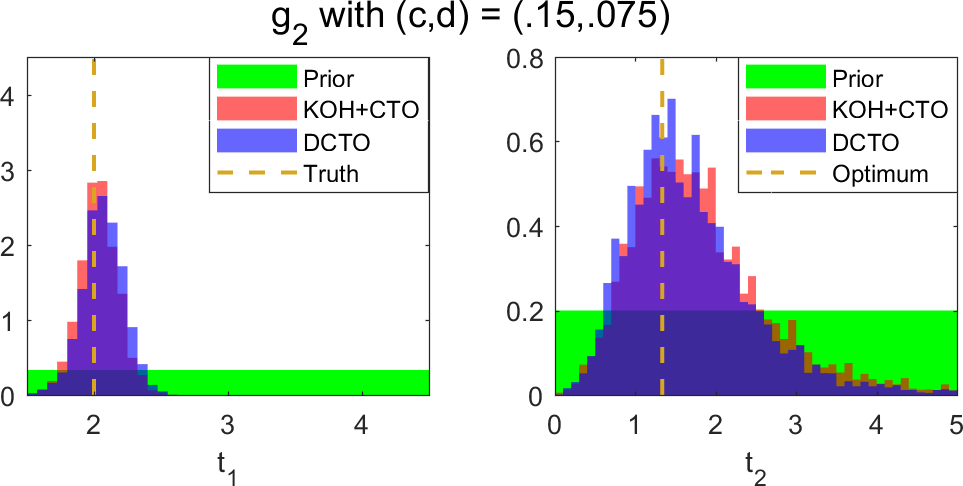
\includegraphics[scale=0.85]{FIG_KOHCTO_DCTO_comp_discrep3_results}
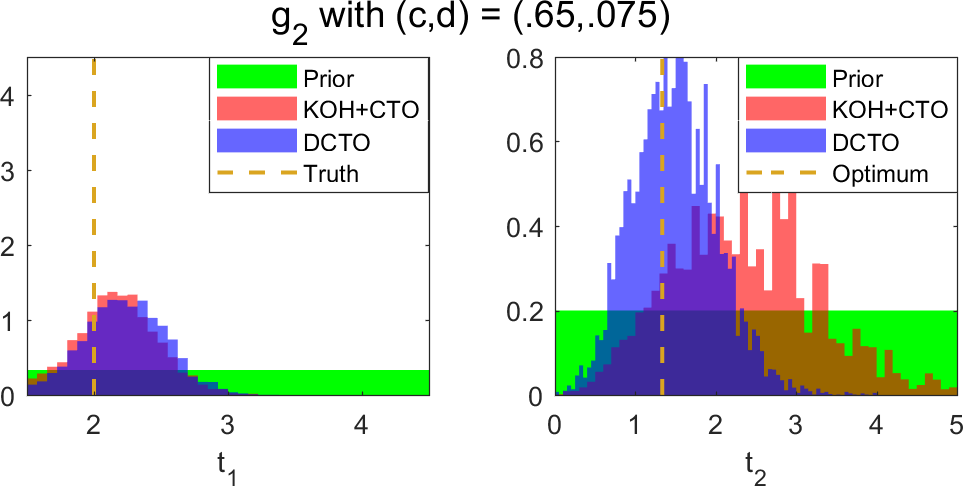
\includegraphics[scale=0.85]{FIG_KOHCTO_DCTO_comp_discrep4_results}
\captionsetup{width=.85\linewidth}
\caption{Prior and posterior distributions of the calibration parameter $\theta_1$ and design parameter $\theta_2$, along with their true/optimal values, for DCTO and KOH+CTO in the case of true systems $g_2$. The top row corresponds to a smaller discrepancy, with $(c,d)=(.15,.075)$; the bottom row corresponds to a larger discrepancy, with $(c,d)=(.65,.075)$.}
\label{fig:2_discrep_results}
\end{figure}
%
Somewhat counterintuitively, even stronger Bayesian learning occurs with respect to $\theta_1$ in the case of $g_1$ than in the case of $g_0$, in each of the two settings of $c$.
%
By contrast, and less surprisingly, the posterior distributions for $\theta_1$ are somewhat wider in the case of $g_2$, for each of the two settings of $(c,d)$.
%
Nonetheless, the posterior distributions for $g_2$, as for $g_0$ and $g_1$, still peak at the true value of $\theta_1$ and at the optimal value of $\theta_2$ under DCTO.
%
The case of $g_2$ with $(c,d)=(.65,.075)$ is the only case in which DCTO and KOH+CTO produce strikingly different results.
%
Here, DCTO supplies a posterior distribution for $\theta_2$ that peaks at the true optimum, while KOH+CTO produces a much wider distribution that fails to peak at the optimum.
%
The reason for this difference is unclear.
%
DCTO and KOH both have fairly high uncertainty in the posterior distribution of $\theta_1$, which propogates to uncertainty in the posterior distribution of $\theta_2$, since the optimal $\theta_2$ is dependent upon the true value of $\theta_1$.
%
It is possible that this affects KOH+CTO more than DCTO since DCTO is able to use the information contained in the true observations of $g_2$ to inform the design of $\theta_2$, whereas under KOH+CTO the true observations are used only in calibration of $\theta_1$ and not in the design of $\theta_2$.
%

%
Matters change in the case of $g_3$, where the calibration procedure is somewhat unsuccessful for both DCTO and KOH+CTO.
%
Figure \ref{fig:3_discrep_results} (upper left) shows that the true value of $\theta_1$ is well into the tails of the posterior distributions.
%
\begin{figure}
\centering
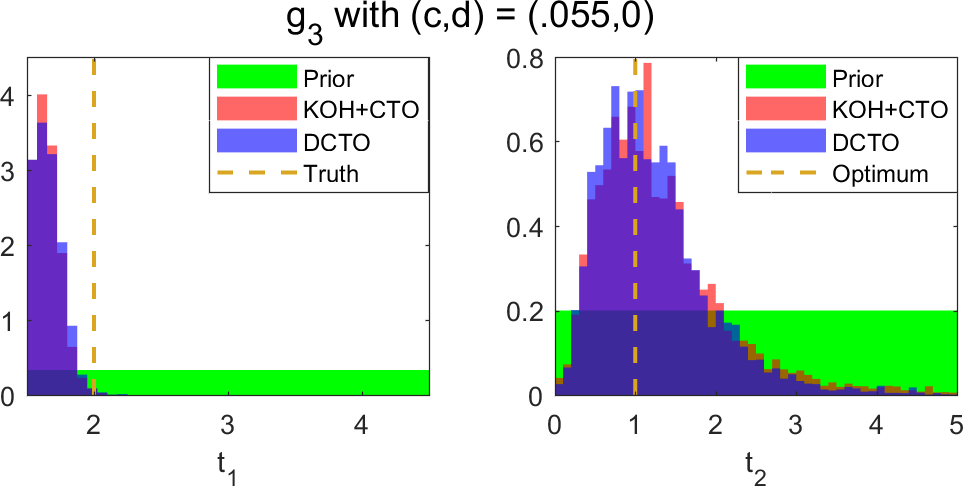
\includegraphics[scale=0.85]{FIG_KOHCTO_DCTO_comp_discrep5_results}
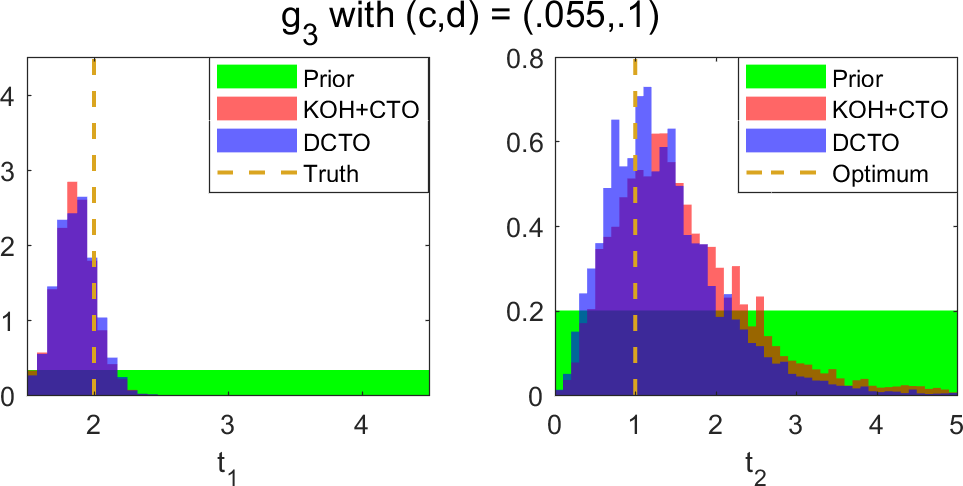
\includegraphics[scale=0.85]{FIG_KOHCTO_DCTO_comp_discrep6_results}
\captionsetup{width=.85\linewidth}
\caption{Prior and posterior distributions of the calibration parameter $\theta_1$ and design parameter $\theta_2$, along with their true/optimal values, for DCTO and KOH+CTO in the case of true systems $g_3$. The top row corresponds to a smaller discrepancy, with $(c,d)=(.055,0)$; the bottom row corresponds to a larger discrepancy, with $(c,d)=(.055,.1)$.}
\label{fig:3_discrep_results}
\end{figure}
%
Surprisingly, increasing $d$ from 0 to 0.1 and keeping $c=0.055$, the results are significantly better, even though the discrepancy in this case is larger.
%
In the lower left of Figure \ref{fig:3_discrep_results}, we see that the posterior distributions again peak sharply near the true value of $\theta_1$.
%
In all versions of the discrepancy function explored here, the posterior distribution under DCTO is roughly similar with respect to $\theta_2$; wider than the posteriors for $\theta_1$, but peaking near the optimal $\theta_2$ even when this is not true of $\theta_1$.
%

%
In order to achieve better results in the case of $g_3$ with $d=0$, we attempted to place a more informative prior on the discrepancy function $\delta_1$.
%
We pursued two different strategies to do this.
%
Firstly, we integrated the discrepancy $g_3-f$ over the supports of $x$ and $t_2$, finding the average value of the discrepancy.
%
We then re-ran DCTO using $m_1(x,t_2)=\left(\int (g_3(z,\theta_1,w)-f(z,\theta_1,w))dzdw\right)/2.5$ as the (constant) mean of the GP prior on $\delta_1$.
%
This corresponds to a case in which one knows on average how far one's model tends to be from the true system.
%
The results, however, were not appreciably different from the original results using a mean of 0 for the GP prior on $\delta_1$.
%
Secondly, we again ran DCTO using $m_1(x,t_2) = g_3(x,\theta_1,t_2)-f(x,\theta_1,t_2)$, so that the GP prior mean on $\delta_1$ was the true discrepancy.
%
This corresponds to a case in which one has (e.g. through extensive experimentation) a more thorough understanding of the form of the model's discrepancy with the true system.
%
This second strategy proved fruitful, producing the results in Figure \ref{fig:3_informative_discrep_results}.
%
\begin{figure}
\centering
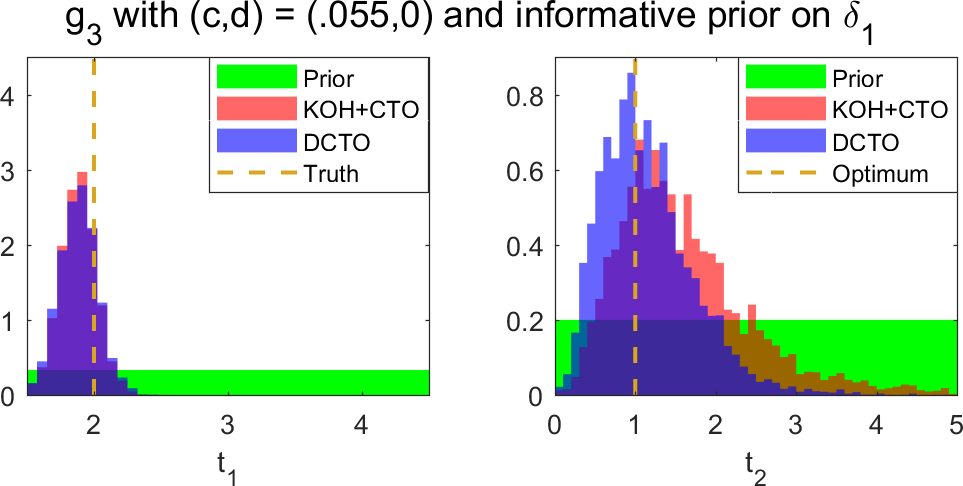
\includegraphics[scale=0.85]{FIG_KOHCTO_DCTO_comp_discrep5_inf_results}
\captionsetup{width=.85\linewidth}
\caption{Prior and posterior distributions of the calibration parameter $\theta_1$ and design parameter $\theta_2$, along with their true/optimal values, for DCTO ond KOH in the case of true systems $g_3$ with $(c,d)=(.055,0)$ and an informative prior for $\delta_1$.}
\label{fig:3_informative_discrep_results}
\end{figure}
%
KOH+CTO and DCTO were equally successful in calibration, but DCTO again outperforms KOH+CTO on design here, with a posterior which is both narrower and more centered on the true optimum.
%
Given that the two design procedures perform similarly with an uninformative prior on $\delta_1$, it's unclear why using an informative prior produces such different design results, especially since the informative prior has an almost identical effect in improving the calibration results in the two cases.
%

%
The posterior predictive distributions under DCTO and KOH+CTO are very close under six of the eight discrepancies studied.
%
Nonetheless, in most of those six cases DCTO enjoys very slightly narrower posterior predictive distributions. 
%
In the two cases under which DCTO and KOH+CTO diverge appreciably, DCTO enjoys much better results, with sharper distributions that center nearer to the true optimal model output.
%
Figure \ref{fig:01_post_dist} shows the posterior predictive distributions for $g_0$, the case of no model discrepancy, and for two settings of $g_1$, the case of multiplicative model discrepancy.
%
\begin{figure}
	\centering
	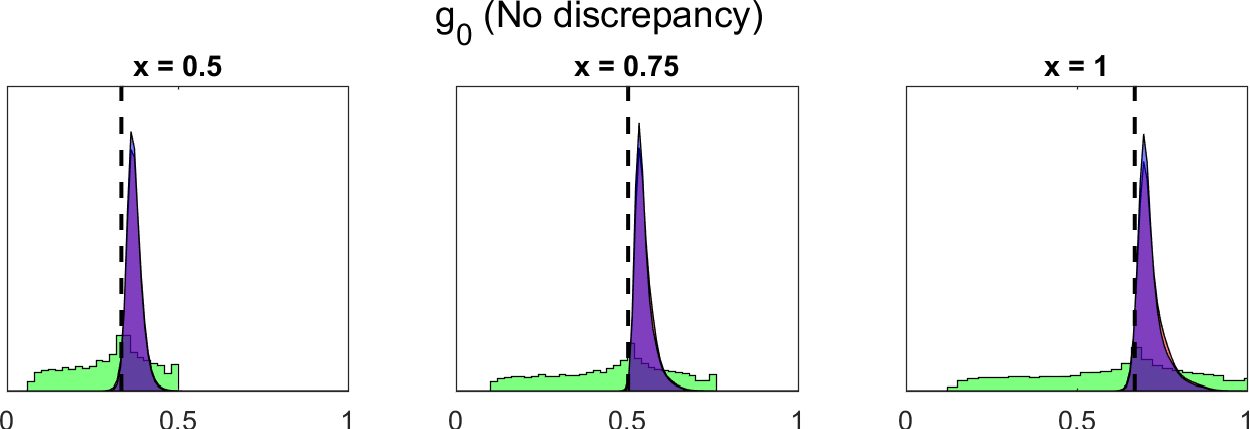
\includegraphics[scale=0.85]{FIG_DCTO_KOHCTO_post_pred_dist_discrep0}\\
	\vspace{1em}
	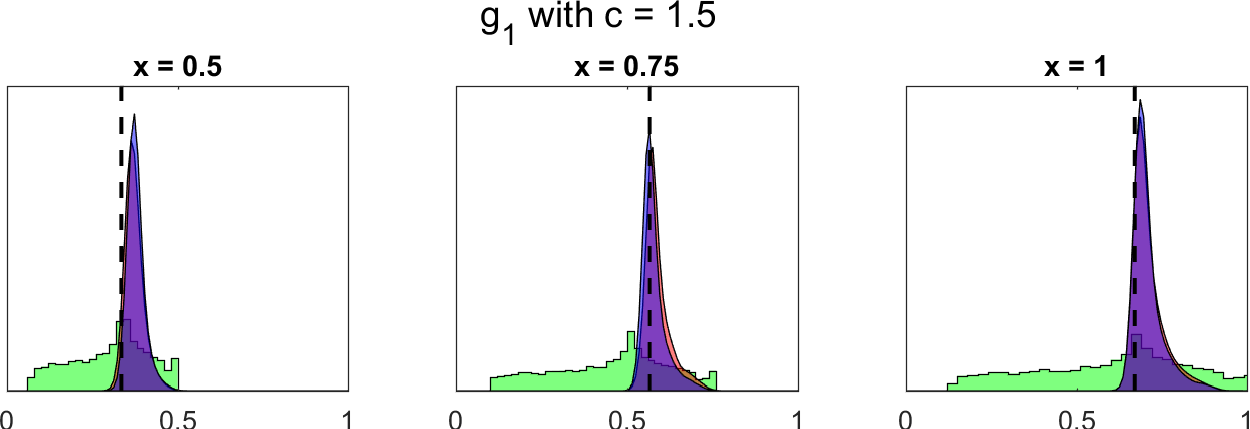
\includegraphics[scale=0.85]{FIG_DCTO_KOHCTO_post_pred_dist_discrep1}\\
	\vspace{1em}
	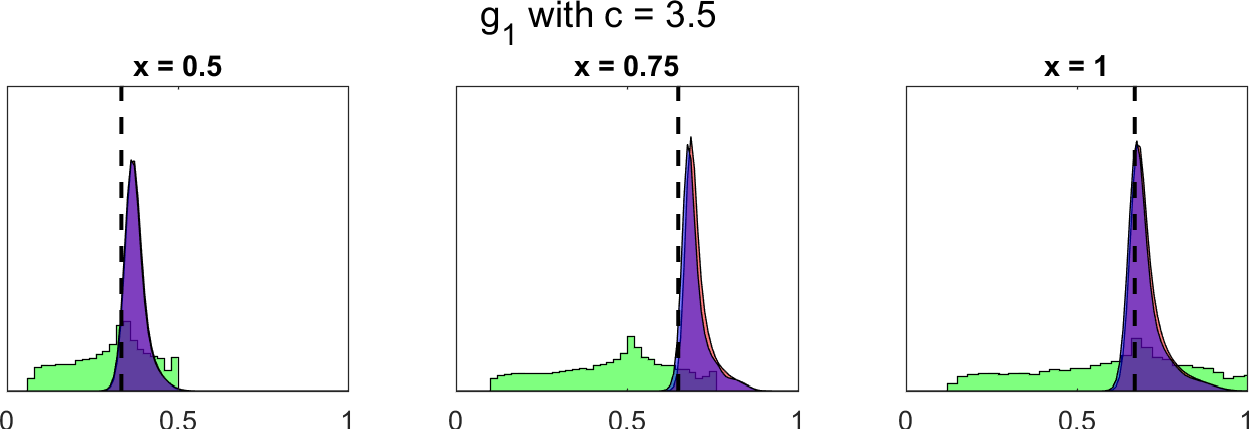
\includegraphics[scale=0.85]{FIG_DCTO_KOHCTO_post_pred_dist_discrep2}
	\captionsetup{width=.85\linewidth}
	\caption{Prior (green) and posterior predictive distributions of the model output, along with the optimum, for DCTO and KOH+CTO at three values of the control input $x$. The red KOH+CTO and blue DCTO distributions overlap almost perfectly, but in all cases except the bottom middle plot, DCTO peaks just slightly above KOH+CTO.}
	\label{fig:01_post_dist}
\end{figure}
%
Here, the posterior predictive distributions for DCTO and KOH+CTO overlap almost perfectly, except for the slightly higher peaks of DCTO.
%

%
Figure \ref{fig:2_post_dist} shows the results for two settings of $g_2$, an additive discrepancy form.
%
For the smaller discrepancy setting of $g_2$, the results are similar to those for $g_0$ and $g_1$, with DCTO enjoying slightly less uncertainty.
%
The larger discrepancy setting for $g_2$ is the same case as that shown in Figure \ref{fig:2_discrep_results}, where KOH+CTO performs well with respect to calibration but poorly with respect to design.
%
Figure \ref{fig:2_post_dist} shows that this poor design corresponds to wildly different predictive performance between DCTO and KOH+CTO, with KOH+CTO suffering from high uncertainty and strange multimodal behavior for some levels of the control input $x$.
%
\begin{figure}
	\centering
	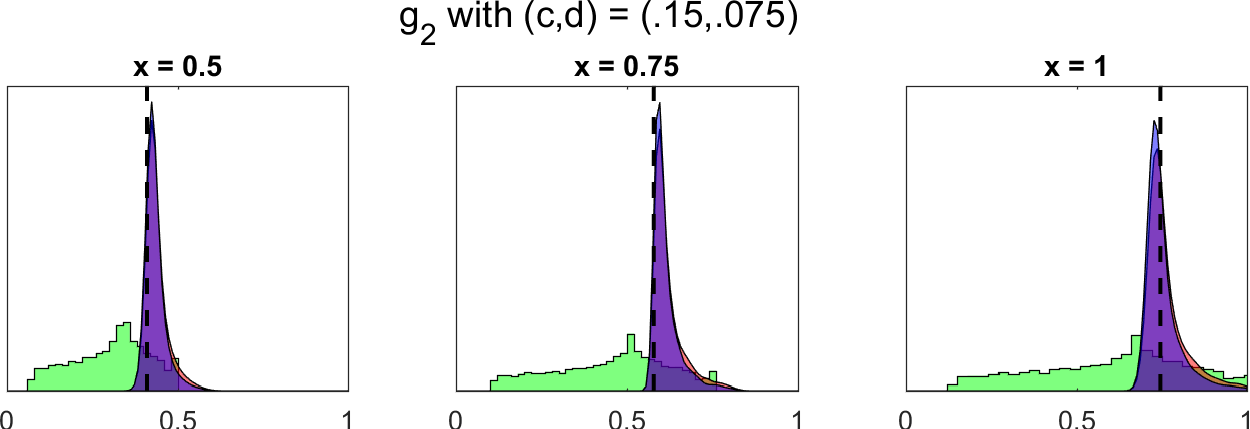
\includegraphics[scale=0.85]{FIG_DCTO_KOHCTO_post_pred_dist_discrep3}\\
	\vspace{1em}
	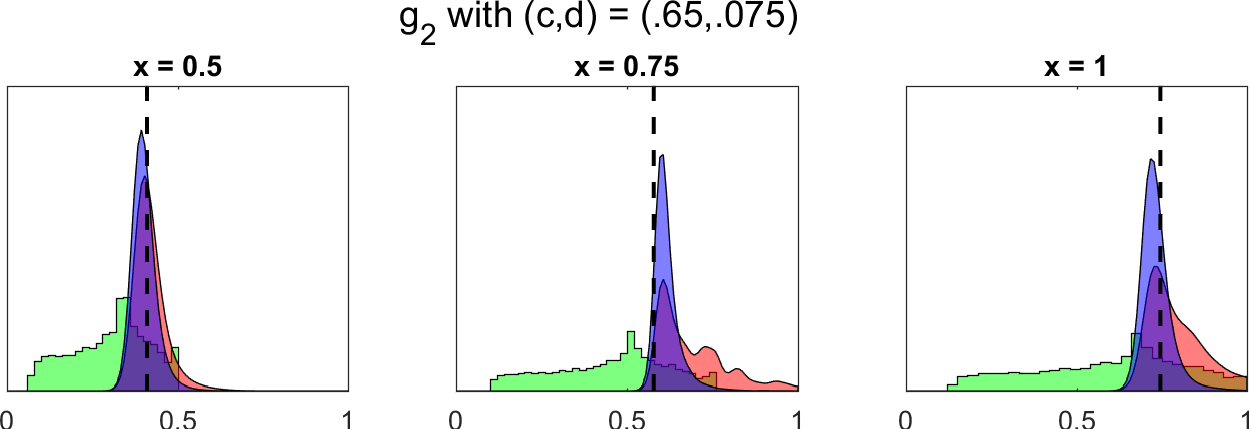
\includegraphics[scale=0.85]{FIG_DCTO_KOHCTO_post_pred_dist_discrep4}
	\captionsetup{width=.85\linewidth}
	\caption{Prior (green) and posterior predictive distributions of the model output, along with the optimum, for DCTO and KOH+CTO at three values of the control input $x$.}
	\label{fig:2_post_dist}
\end{figure}
%
It is however notable that even here, the posterior predictive distribution's global mode still occurs at the same location as the global mode under DCTO, despite the fact that this is not true of the posterior distributions of the design parameter $t_2$ under the two techniques.
%

The additive discrepancy form of $g_3$ again has similar posterior predictive results under DCTO and KOH+CTO for both small and large versions of the discrepancy, except when an informative prior is supplied for the discrepancy function.
%
Recall that the small discrepancy version of $g_3$ is a case in which both DCTO and KOH performed poorly with respect to calibration, as shown in Figure \ref{fig:3_discrep_results}.
%
The top row of Figure \ref{fig:3_post_dist} shows that this poor calibration does not result in similarly poor predictive performance.
%
The improved calibration that results from applying an informative prior, as shown in Figure \ref{fig:3_informative_discrep_results}, inflates the posterior uncertainty surrounding the design variable $t_2$ for KOH+CTO, while slightly deflating the $t_2$ uncertainty for DCTO.
%
Figure \ref{fig:3_post_dist} (middle row) seems to show that this difference between KOH+CTO translates to similar differences in posterior predictive distributions when using the informative prior: slightly less uncertainty under DCTO, slightly more under KOH+CTO.
%
However, despite the fact that both techniques experience dramatically better calibration under the informative prior than without it, there is not a similarly dramatic difference between the posterior predictive distributions with and without the informative prior, under either technique.
%
The flexibility of the discrepancy term in CTO allows for accurate prediction even when the calibration is inaccurate.
%
\begin{figure}
	\centering
	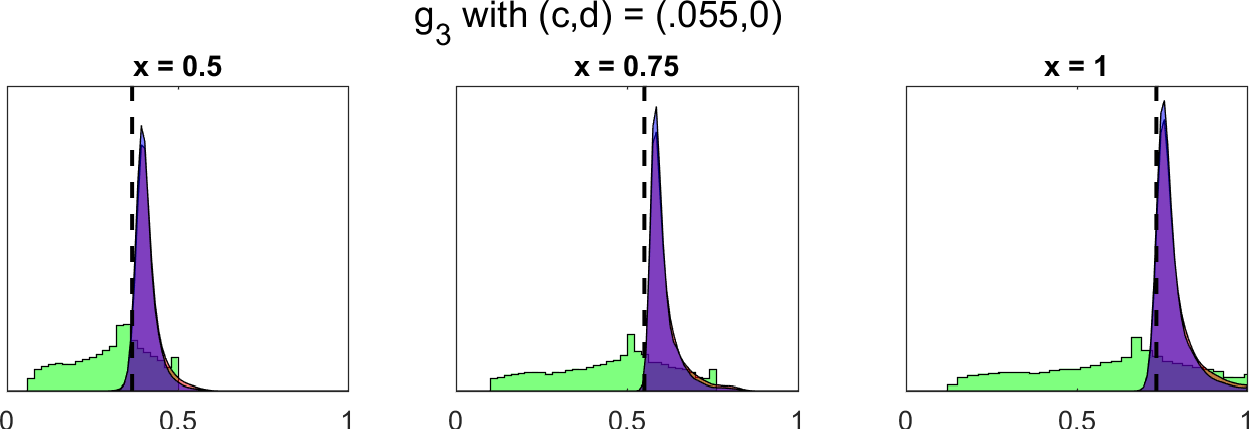
\includegraphics[scale=0.85]{FIG_DCTO_KOHCTO_post_pred_dist_discrep5}\\
	\vspace{1em}
	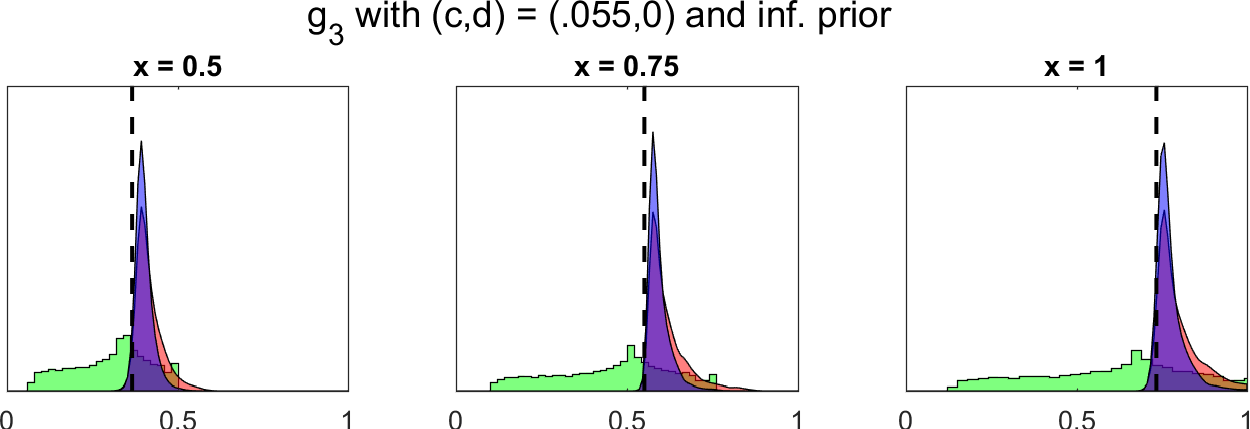
\includegraphics[scale=0.85]{FIG_DCTO_KOHCTO_post_pred_dist_discrep5_inf}\\
	\vspace{1em}
	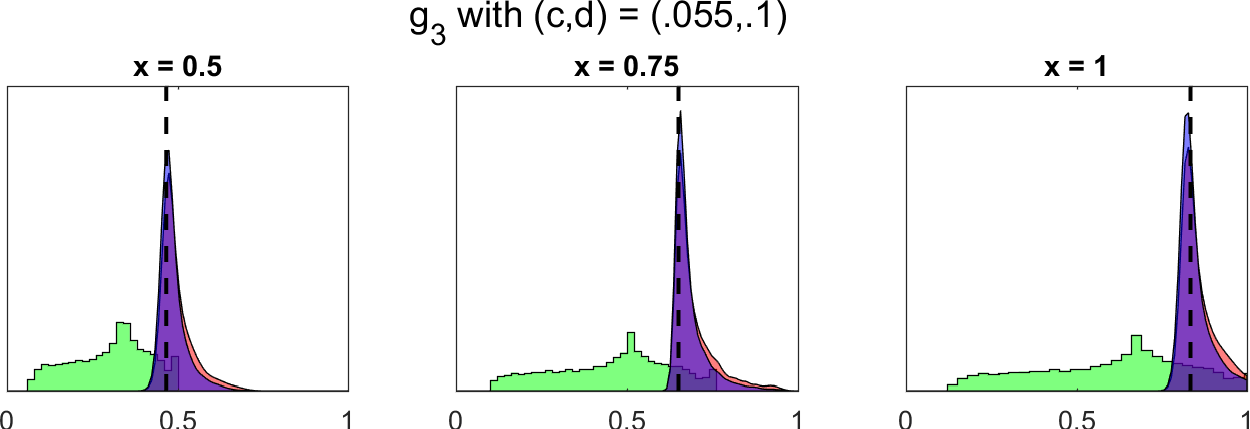
\includegraphics[scale=0.85]{FIG_DCTO_KOHCTO_post_pred_dist_discrep6}
	\captionsetup{width=.85\linewidth}
	\caption{Prior (green) and posterior predictive distributions of the model output, along with the optimum, for DCTO and KOH+CTO at three values of the control input $x$.}
	\label{fig:3_post_dist}
\end{figure}
%

%
The calibration, design, and predictive results for all seven cases (one case of zero discrepancy plus two versions each of three different forms of discrepancy) are summarized in Table \ref{table:vars_and_ads}.
%
The top table shows the posterior variances of the calibration parameter $t_1$, the design parameter $t_2$, and the predictive distribution $\tilde y$ at control setting $x=0.75$.
%
The bottom table shows the absolute deviation of the resulting posterior means $\widehat{\theta_1},\widehat{\theta_2},$ and $\hat{\tilde y}$ from their known true values.
\begin{table}[]
\centering
\begin{tabular}{l|cc|cc}
&\multicolumn{2}{c|}{$t_1$ variance}&
\multicolumn{2}{c}{$t_2$ variance} \\ \hline
Discrepancy    & DCTO   & KOH+CTO & DCTO    & KOH+CTO   \\ \hline
0              & 0.0198 & 0.0179 & 0.6636 & 0.7066\\ \hline
1, small       & 0.0181 & 0.0131 & 0.5881 & 0.7055\\ \hline
1, large       & 0.0129 & 0.0096 & 0.7676 & 0.7465\\ \hline
2, small       & 0.0233 & 0.0209 & 0.5849 & 0.7022\\ \hline
2, large       & 0.0896 & 0.0872 & 0.2711 & 0.7992\\ \hline
3, small       & 0.0108 & 0.0093 & 0.4903 & 0.6257\\ \hline
3, large       & 0.0216 & 0.0207 & 0.5228 & 0.7009\\ \hline
3, small, inf. & 0.0201 & 0.0179 & 0.3330 & 0.6787\\ \hline
\end{tabular}\\
\vspace{.25in}
\begin{tabular}{l|cc|cc}
&\multicolumn{2}{c|}{$|\theta_1-\widehat{\theta_1}|$} & \multicolumn{2}{c}{$|\theta_2-\widehat{\theta_2}|$}\\ \hline
Discrepancy    & DCTO    & KOH+CTO & DCTO    & KOH+CTO \\ \hline
0              & 0.0969 & 0.1124 & 0.2594 & 0.2838\\ \hline
1, small       & 0.0007 & 0.0427 & 0.2720 & 0.3816\\ \hline
1, large       & 0.0436 & 0.0001 & 0.3614 & 0.4361\\ \hline
2, small       & 0.0686 & 0.0353 & 0.3365 & 0.4664\\ \hline
2, large       & 0.2346 & 0.1808 & 0.1577 & 1.0270\\ \hline
3, small       & 0.3393 & 0.3464 & 0.2304 & 0.3090\\ \hline
3, large       & 0.1325 & 0.1403 & 0.3651 & 0.5781\\ \hline
3, small, inf. & 0.1151 & 0.1157 & 0.1488 & 0.5921\\ \hline
\end{tabular}
\caption{Posterior variances and mean absolute deviations for the calibration variable $\theta_1$ and the design variable $\theta_2$. The estimator $\widehat{\theta_i}$ is the posterior mean of $t_i$. The final line in each table gives the results for the use of an informative prior for the discrepancy of $g_3$ with $(c,d)=(0,.055)$.} 
\label{table:vars_and_ads}
\end{table}
%
It appears that KOH produces narrower calibration posteriors than DCTO, as the variances for $\theta_1$ are uniformly lower for KOH, if usually only slightly.
%
However, when we instead look at $|\theta_1-\widehat{\theta_1}|$, matters are less clear.
%
DCTO has a lower calibration estimate absolute error in five of the eight cases studied here, and in general, the differences between the two procedures here is small.
%
It thus appears that DCTO and KOH+CTO enjoy similar levels of success in calibration.
%
Clearer differences emerge in looking at the performance of the two procedures with respect to the design variable.
%
DCTO produces a smaller posterior variance in seven out of the eight cases, in two cases more than halving the variance produced under KOH+CTO.
%
The difference is even more pronounced for $|\theta_2-\widehat{\theta_2}|$ under the two procedures, as DCTO produces a lower absolute error in each of the eight cases, sometimes strikingly so.
%
For example, in the large discrepancy version of $g_2$, DCTO produces an estimate with less than one sixth the absolute error of KOH+CTO.
%
It appears that DCTO and KOH+CTO perform similarly with respect to calibration, but that DCTO produces superior results with respect to design.
%


\bigskip

%\begin{center}
%{\large\bf SUPPLEMENTARY MATERIAL}
%\end{center}
%
%\begin{description}
%
%\item[Title:] Brief description. (file type)
%
%\item[R-package for  MYNEW routine:] R-package �MYNEW� containing code to perform the diagnostic methods described in the article. The package also contains all datasets used as examples in the article. (GNU zipped tar file)
%%
%\item[HIV data set:] Data set used in the illustration of MYNEW method in Section~ 3.2. (.txt file)
%
%\end{description}

\bibliographystyle{Chicago}

\bibliography{lit_review}
\end{document}

\begin{figure}
\begin{center}
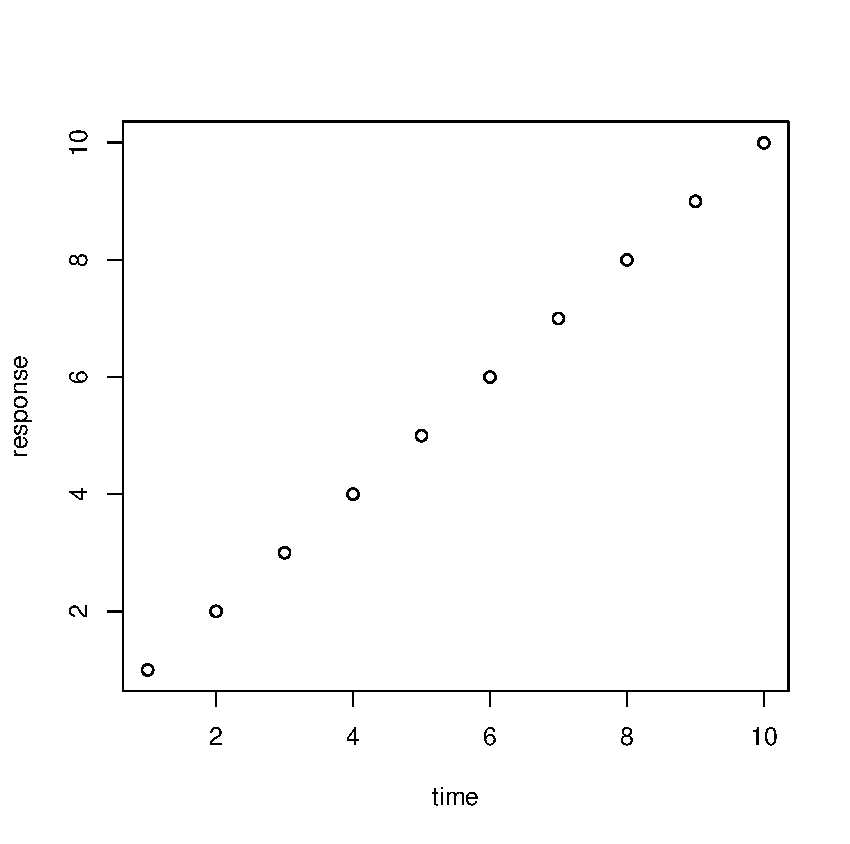
\includegraphics[width=3in]{fig1.pdf}
\end{center}
\caption{Consistency comparison in fitting surrogate model in the tidal
power example. \label{fig:first}}
\end{figure}

\begin{table}
\caption{D-optimality values for design $X$ under five different scenarios.  \label{tab:tabone}}
\begin{center}
\begin{tabular}{rrrrr}
one & two & three & four & five\\\hline
1.23 & 3.45 & 5.00 & 1.21 & 3.41 \\
1.23 & 3.45 & 5.00 & 1.21 & 3.42 \\
1.23 & 3.45 & 5.00 & 1.21 & 3.43 \\
\end{tabular}
\end{center}
\end{table}

\begin{itemize}
\item Note that figures and tables (such as Figure~\ref{fig:first} and
Table~\ref{tab:tabone}) should appear in the paper, not at the end or
in separate files.
\item In the latex source, near the top of the file the command
\verb+\newcommand{\blind}{1}+ can be used to hide the authors and
acknowledgements, producing the required blinded version.
\item Remember that in the blind version, you should not identify authors
indirectly in the text.  That is, don't say ``In Smith et. al.  (2009) we
showed that ...''.  Instead, say ``Smith et. al. (2009) showed that ...''.
\item These points are only intended to remind you of some requirements.
Please refer to the instructions for authors
at \url{http://www.tandfonline.com/action/authorSubmission?journalCode=utch20&page=instructions#.UieFdDafgx0}
\item If you have Supplementary Material (eg software, data, technical
proofs), identify them in the section below.  In early stages of the
submission process, you may be unsure what to include as supplementary
material.  Don't worry---this is something that can be worked out at later stages.
\end{itemize}
